\section{Method}
While it relies on the same principles as \cite{caldarelli2012network}, our proposed model is conceptually different in that our "products" are Wikipedia articles, which are not the basis for competitions but rather for cooperation. In the economics literature product ubiquity is taken to be product "disvalue"- rarer is better. In our case editors enrich the articles together to make best articles. So article ubiquity - touched by many editors - could be take as value.  However, like countries, editors have limited capabilities and limited resources (e.g., time), which force them make choices on their contributions, so for behavioural reasons they may chose to work on less ubiquitous articles.

\begin{figure*}[!t]
\centering
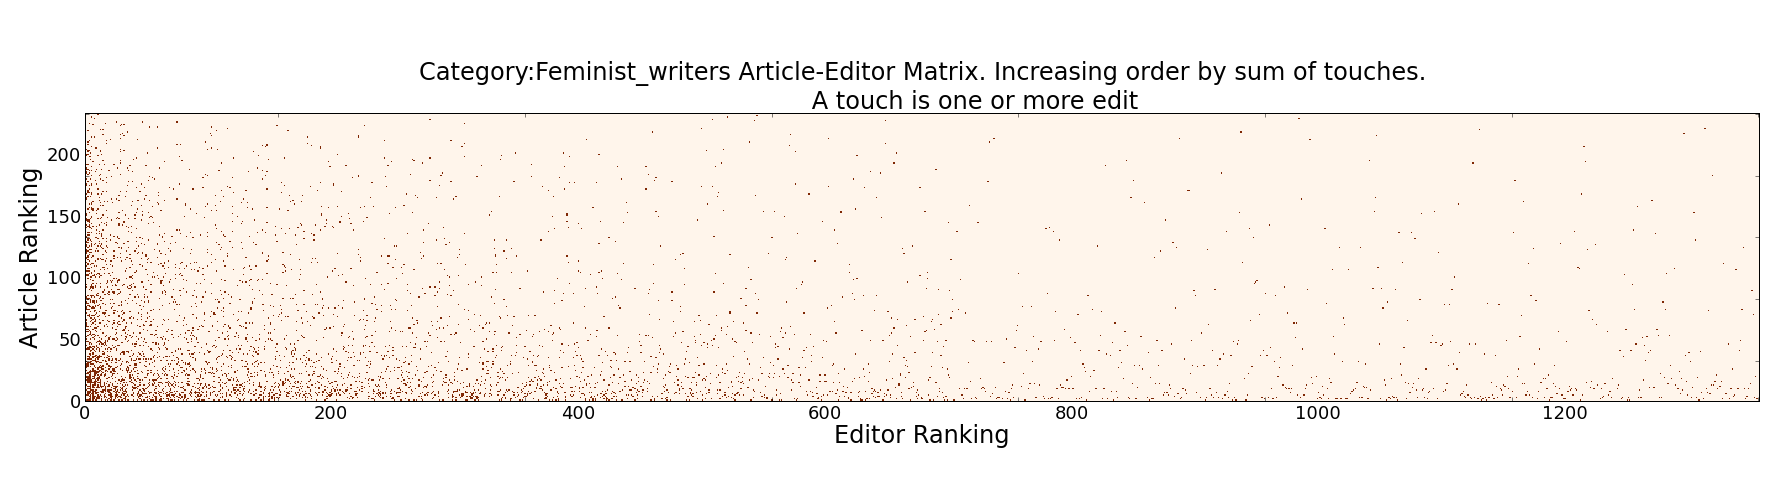
\includegraphics[width=2.0\columnwidth]{Figures/Category_Feminist_writerstriangle_matrix_corrected.png}
\caption{Typical $\mathbf{M}$ matrix for a Wikipedia category (here, {\it Feminist Writers}) ordered on both dimensions by descending order of number of articles modified by an editor (horizontal axis) and of number editors who have modified an article (vertical axis). The structure of $\mathbf{M}$ is triangular and shows that some editors have a pervasive activity over articles, while most editors edit only a few. Similarly, some articles receive widespread attention by editors, while most articles are modified only by a few editors.}
\label{fig:triangle}
\end{figure*}

\begin{figure}[!t]
\centering
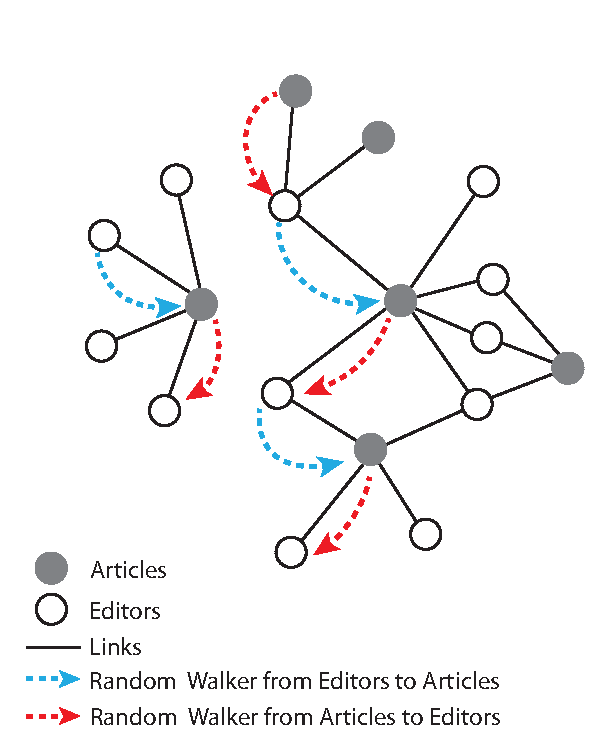
\includegraphics[width=0.7\columnwidth]{Figures/bi-partite_net.eps}.
\caption{}
\label{fig:convergence}
\end{figure}


A matrix $\mathbf{M}$, between editors and articles in Wikipedia category is defined to be $1$ when an article has a contribution by a given editor and $0$ otherwise. The example shown in \ref{fig:triangle} displays the matrix ordered on both dimensions by decreasing order of editors who have changed more articles (vertical axis) and by decreasing order of articles that have been changed by most editors (horizontal axis) for a category of Wikipedia articles (here Category:Feminist Writers). The matrix describes the activity of an editor in the given category by the sum of articles contributed to; and the attention an article has received from editors by the sum of editors contributing to it. 

\begin{equation}
\begin{cases}
 k_{e}^{(0)} = \sum_{a=1}^{N_{a}}\\
 k_{a}^{(0)} = \sum_{e=1}^{N_{N_{e}}}
\end{cases}
\label{HHinit}
\end{equation}

Now, let's consider the second iteration:  if an article has been changed by editors who edited more articles, then the quality of the article should be higher. The claim is that power users confer value. Similarly, if an editor has edited articles that have been edited by more editors, then the expertise of the editor should be higher (a reason for making this claim is the collaborative nature of Wikipedia as you interact with more editors you learn the "Wikipedia process" more, and are fitter at editing Wikipedia, not necessarily at writing in general). 
Accordingly, the third iteration is the following: if an article has been changed by editors who edited more articles that have edited by more editors, then the quality of the article should be higher. Similarly, if an editor has edited articles that have been edited by more editors that have edited more articles, then the expertise of the editor should be higher. Although the interpretation is difficult to imagine passed this iteration, the algorithm goes on recursively, incorporating the quality (resp. expertise) information of the article (resp. editor) at the previous iteration.

A natural question is if this process is potentially infinite. Our goal is to rank editors and articles in relation to each other within the group, so the question is reduced to whether the ranking converges. As is, the algorithm
has a "major problem in the algorithm is that it is a case of a
consensus dynamics i.e. the state of a node at iteration $n$ is just
the average of the state of its neighbors at iteration $n+1$. It is well
known that such iterations have the uniform state (all the nodes
equal) as the natural fixpoint." \cite{caldarelli2012network}

To gain useful information Caldarelli et al. introduce nonlinear biases so that "neighbors" are not all treated equally. The algorithm at iteration $n$ is then written as:

\begin{equation}
\begin{cases}
 \mathbf{w}^{(n+1)}_e (\alpha,\beta) = \sum_{a=1}^{N_a}  \mathbf{G}_{ea}(\beta) \mathbf{w}^{(n)}_a (\alpha,\beta)\\
\mathbf{w}^{(n+1)}_a (\alpha,\beta) = \sum_{e=1}^{N_e}  \mathbf{G}_{ae}(\beta) \mathbf{w}^{(n)}_e (\alpha,\beta)\\
\end{cases}
\label{random_walker}
\end{equation}

where the Markov transition matrix $\mathbf{\hat{G}}$ is given by 

\begin{equation}
\begin{cases}
\mathbf{G}_{ea}(\beta) = \frac{\mathbf{M}_{ea} \mathbf{k}_{e}^{-\beta}}{\sum_{e' = 1}^{N_e} \mathbf{M}_{e'a} \mathbf{k}_{e'}^{-\beta}}\\
\mathbf{G}_{ae}(\alpha) = \frac{\mathbf{M}_{ea} \mathbf{k}_{a}^{-\alpha}}{\sum_{a' = 1}^{N_a} \mathbf{M}_{ea'} \mathbf{k}_{a'}^{-\alpha}}\\
 \end{cases}
\end{equation}

Here $\mathbf{G_{ea}}$ gives the probability to jump from article $a$ to editor $e$ in a single step, and $\mathbf{G_{ae}}$ the probability to jump from editor $e$ to article $a$ also in a single step. We shall give more insights on how $\alpha$ and $\beta$ influence the random walker by analyzing the transition matrices $\mathbf{G}_{ea}(\beta)$ and $\mathbf{G}_{ae}(\alpha)$. The transition matrices depend only from the initial conditions $\mathbf{M}$ and $k_e$ and $k_a$ given by (\ref{HHinit}). Since both transition matrices have the same structure, we only explain the intuition for  $\alpha$ and $\mathbf{G}_{ae}(\alpha)$. $\alpha$ is the power exponent of the inverse of $k_a$, and therefore the bias depends on the possible values taken by $\alpha$. If $\alpha = 0$, we recover the zero\textsuperscript{th} order iteration. For $\alpha > 0$, the probability to jump from editor $e$ to article $a$ is weighted by a concave function of the sum of editors who have modified the article. The larger $\alpha$ the less the number of editors is important to an article. On the contrary, if $\alpha < 0$ the probability to jump from an editor to an article is a positive function of the sum of editors who have modified the article. For $-1 < \alpha < 0$, the function is concave, while for $\alpha < -1$, the function is convex, which means that the more editors, the even more the weight on the article. The same considerations hold for $\beta$ and the probability $\mathbf{G}_{ea}$ to jump from an article to an editor.

A ranking-by-iteration plot shows how the ranking typically converges over iterations. As shown in Figure \ref{fig:convergence}, the algorithm converges in a non-trivial way as they can be reduced ergodic Markov chains \cite{caldarelli2012network}. In the iterative solution we see how certain editors start low, but then climb in rankings. This means that they are editing few articles, but those articles are of edited more by other users - our proxy so far for higher quality. Likewise there are some users who fall in rankings, which are those who edit a lot of articles, but the articles they edit are not edited by many others.

A property of this algorithm, is that with the following balance condition,

\begin{equation}
\mathbf{G}_{ae} \mathbf{w}^*_e = \mathbf{G}_{ea} \mathbf{w}^*_a
\end{equation}

which can be rewritten as,

\begin{equation}
\begin{cases}
\mathbf{w}^{*}_{e} \sim \mathbf{k}^{1-\beta}_{e} \langle \mathbf{k}_{a}^{-\alpha}\rangle_e \\
\mathbf{w}^{*}_{a} \sim \mathbf{k}^{1-\alpha}_{a} \langle \mathbf{k}_{e}^{-\beta}\rangle_a
\end{cases} \label{eqsim}
\end{equation}



it is the analytical formulation we use onwards. It is important to note a crucial difference in the way we apply the weighted random walk model in the case of open collaboration compared to the countries-products problem. In \cite{caldarelli2012network}, $w^*_p$ is a measure of ubiquity (i.e. dis-quality) because many countries can sell the product, while here $w^*_a$ is also a measure of ubiquity in the sense that many editors have modified the article. In the case of open collaboration, $w^*_a$ is a measure of quality.

\begin{figure}[!t]
\centering
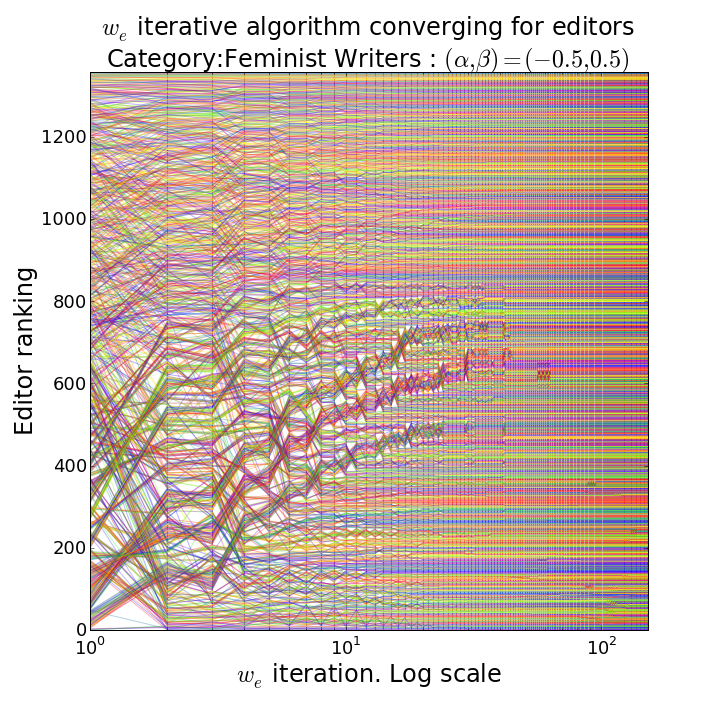
\includegraphics[width=0.9\columnwidth]{Figures/fem_editors_iter_converge.png}.
\caption{Convergence of $w_e$}
\label{fig:convergence}
\end{figure}




Our aim here is to calibrate $\alpha$ and $\beta$ for various categories of articles on Wikipedia against some exogenous metrics of editors' expertise and articles' quality, to understand how the biases can inform on the emergence of respectively expertise and quality.